\subsubsection{Basic Operations}
\begin{lstlisting}[basicstyle=\small]
octave:1> a = pi
a =  3.1416
octave:2> disp(sprintf('6 decimals: %0.6f', a))
6 decimals: 3.141593
octave:3> a
a =  3.1416
octave:4> format long
octave:5> a
a =  3.141592653589793
octave:6> format short
octave:7> a
a =  3.1416
octave:8> v = 1:0.1:2
v =

    1.0000    1.1000    1.2000    1.3000    1.4000    1.5000    1.6000    1.7000    1.8000    1.9000    2.0000

octave:9> v = 1:0.1:2
v =

 Columns 1 through 8:

    1.0000    1.1000    1.2000    1.3000    1.4000    1.5000    1.6000    1.7000

 Columns 9 through 11:

    1.8000    1.9000    2.0000

octave:10> v = 1:6
v =

   1   2   3   4   5   6

octave:11> zeros(1,3)
ans =

   0   0   0

octave:12> rand(1,3)
ans =

   0.43623   0.76554   0.23635

octave:13> randn(1,3)
ans =

   0.5602642  -0.0043628   0.1344922

octave:14> w = -6 + sqrt(10)*(randn(1,10000))

octave:15> hist(w)
\end{lstlisting}

\begin{figure}[h]
  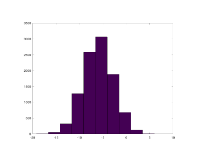
\includegraphics[width=4cm, height=3cm]{hist.png}
\end{figure}

\begin{lstlisting}[basicstyle=\small]
octave:1> w = -6 + sqrt(10)*(rand(1,10000));

octave:2> hist(w,50)
\end{lstlisting}

\begin{figure}[h]
  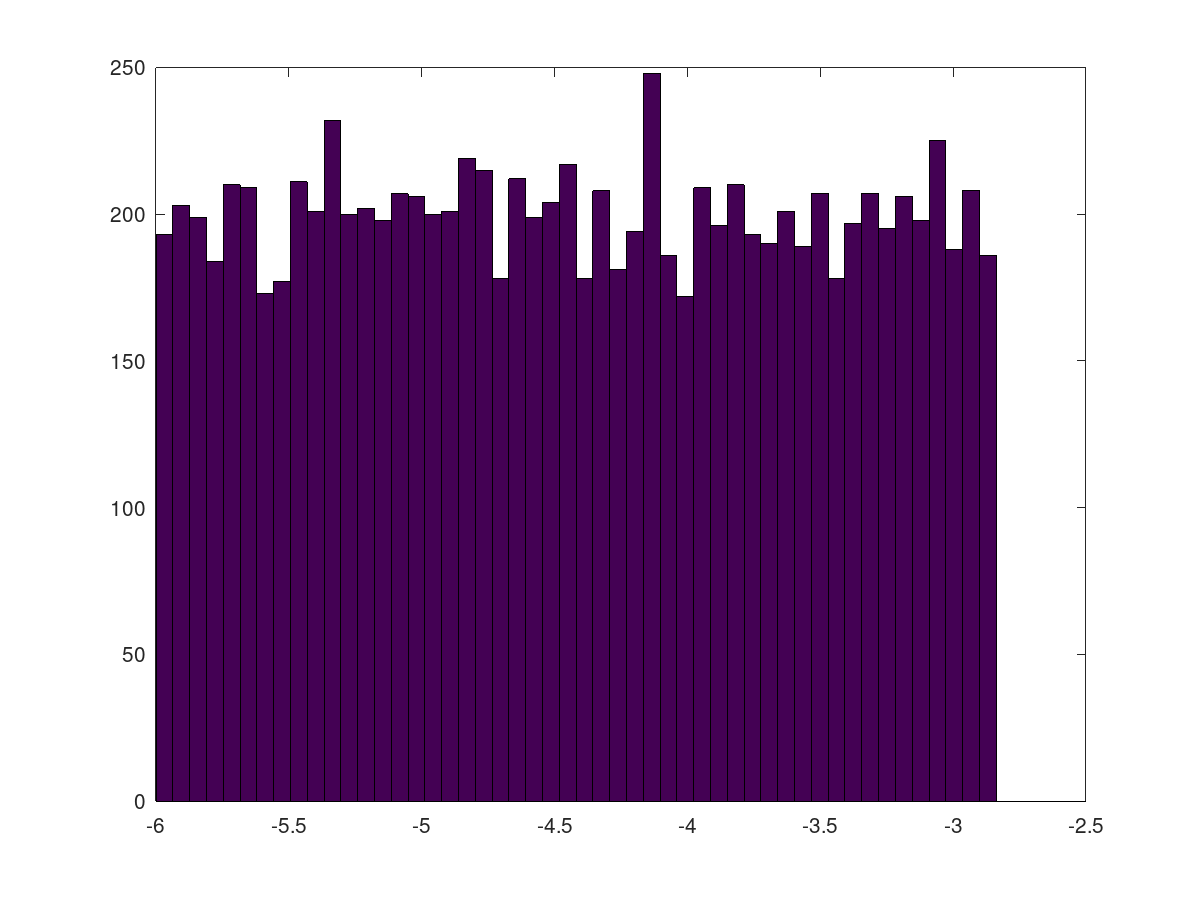
\includegraphics[width=4cm, height=3cm]{hist2.png}
\end{figure}

\subsubsection{Moving Data around}
\begin{lstlisting}[basicstyle=\small]
octave:1> A = [1,2;3,4;4,5]
A =

   1   2
   3   4
   4   5

octave:2> size(A)
ans =

   3   2

octave:3> sz = size(A)
sz =

   3   2

octave:4> size(sz)
ans =

   1   2

octave:5> size(A,1)
ans =  3
octave:6> size(A,2)
ans =  2
octave:7> length(A)
ans =  3
octave:8> length([1,2,3,4,5])
ans =  5
octave:9> 
octave:9> 
octave:9> pwd
ans = /home/sahasra
octave:10> cd /home/sahasra/
octave:11> pwd
ans = /home/sahasra
octave:12> ls
Android          Documents   Music     Public     Videos
AndroidStudioProjects  Downloads   MyPaint   snap
Desktop          examples.desktop  Pictures  Templates
octave:13> who
Variables in the current scope:

A    ans  sz

octave:14> whos
Variables in the current scope:

   Attr Name        Size                     Bytes  Class
   ==== ====        ====                     =====  ===== 
        A           3x2                         48  double
        ans         1x13                        13  char
        sz          1x2                         16  double

Total is 21 elements using 77 bytes

octave:15> clear
octave:16> whos
octave:17> A = [1,2;3,4;5,6]
A =

   1   2
   3   4
   5   6

octave:18> A(3,2)
ans =  6
octave:19> A(2,:)
ans =

   3   4

octave:20> A(:,2)
ans =

   2
   4
   6

octave:21> A([1,3], :)
ans =

   1   2
   5   6

octave:22> A([2,3], :)
ans =

   3   4
   5   6

octave:23> A(:,2) = [10;11;12]
A =

    1   10
    3   11
    5   12

octave:24> A = [A, [5;6;7]]
A =

    1   10    5
    3   11    6
    5   12    7

octave:25> A(:)
ans =

    1
    3
    5
   10
   11
   12
    5
    6
    7

octave:26> A
A =

    1   10    5
    3   11    6
    5   12    7

octave:27> B = [45;46;47]
B =

   45
   46
   47

octave:28> C = [A,B]
C =

    1   10    5   45
    3   11    6   46
    5   12    7   47


\end{lstlisting}


\subsubsection{Computing on Data}
\begin{lstlisting}[basicstyle=\small]
octave:1> A = [1 2;3 4;5 6]
A =

   1   2
   3   4
   5   6

octave:2> B = [11 12; 13 14; 15 16]
B =

   11   12
   13   14
   15   16

octave:3> C = [1  1; 2 2]
C =

   1   1
   2   2

octave:4> A*C
ans =

    5    5
   11   11
   17   17

octave:5> A .* B % A .* B gives element wise operation
ans =

   11   24
   39   56
   75   96

octave:6> 1 ./ A
ans =

   1.00000   0.50000
   0.33333   0.25000
   0.20000   0.16667

octave:7> v = [1;2;3]
v =

   1
   2
   3

octave:8> log(v)
ans =

   0.00000
   0.69315
   1.09861

octave:9> exp(v)
ans =

    2.7183
    7.3891
   20.0855

octave:10> abs([-1; 2; -3])
ans =

   1
   2
   3

octave:11> A
A =

   1   2
   3   4
   5   6

octave:12> A' % A' = A transpose
ans =

   1   3   5
   2   4   6

octave:13> val = max([1;2;3;6;7])
val =  7
octave:14> max(A)
ans =

   5   6

octave:15> A
A =

   1   2
   3   4
   5   6

octave:16> a = [1;4;6;7;9]
a =

   1
   4
   6
   7
   9

octave:17> a < 3
ans =

  1
  0
  0
  0
  0

octave:18> find(a<3)
ans =  1
octave:19> A = magic(3) % Magic Square
A =

   8   1   6
   3   5   7
   4   9   2

octave:20> [r,c] = find(a >= 7)
r =

   4
   5

c =

   1
   1

octave:21> a
a =

   1
   4
   6
   7
   9

octave:22> a = a'
a =

   1   4   6   7   9

octave:23> sum(a)
ans =  27
octave:24> rand(3)
ans =

   0.272471   0.059338   0.757392
   0.414497   0.174242   0.354694
   0.811891   0.935437   0.956667

octave:25> A
A =

   8   1   6
   3   5   7
   4   9   2

octave:26> max(A,[],1)
ans =

   8   9   7

octave:27> max(A,[],2)
ans =

   8
   7
   9

octave:28> max(max(A))
ans =  9
octave:29> A
A =

   8   1   6
   3   5   7
   4   9   2

octave:30> pinv(A)
ans =

   0.147222  -0.144444   0.063889
  -0.061111   0.022222   0.105556
  -0.019444   0.188889  -0.102778

octave:31> temp = pinv(A)
temp =

   0.147222  -0.144444   0.063889
  -0.061111   0.022222   0.105556
  -0.019444   0.188889  -0.102778


octave:32> temp * A
ans =

   1.0000e+00   2.0817e-16  -3.1641e-15
  -6.1062e-15   1.0000e+00   6.2450e-15
   3.0531e-15   4.1633e-17   1.0000e+00

octave:33> % this is the 3x3 Identity matrix, 
           % not having exact values beacuse of variable overflow
\end{lstlisting}

\begin{lstlisting}[basicstyle=\small]
octave:1> t = [0:0.01:0.98];
octave:2> y1 = sin(2*pi*4*t);
octave:3> plot(t,y1)
\end{lstlisting}

\begin{figure}[h]
  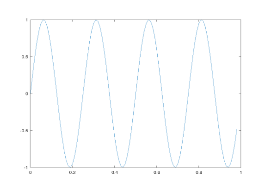
\includegraphics[width=6cm, height=4cm]{sineplot.png}
\end{figure}

\begin{lstlisting}[basicstyle=\small]

octave:4> y2 = cos(2*pi*4*t);
octave:5> plot(t,y1);
octave:6> hold on;
octave:7> plot(t, y2, 'r');
octave:8> xlabel('time')
octave:9> ylabel('value')
octave:10> legend('sin', 'cos')
octave:11> title('sine-cosine plot')
octave:12> print -dpng 'myPlot.png'
\end{lstlisting}

\begin{figure}[h]
  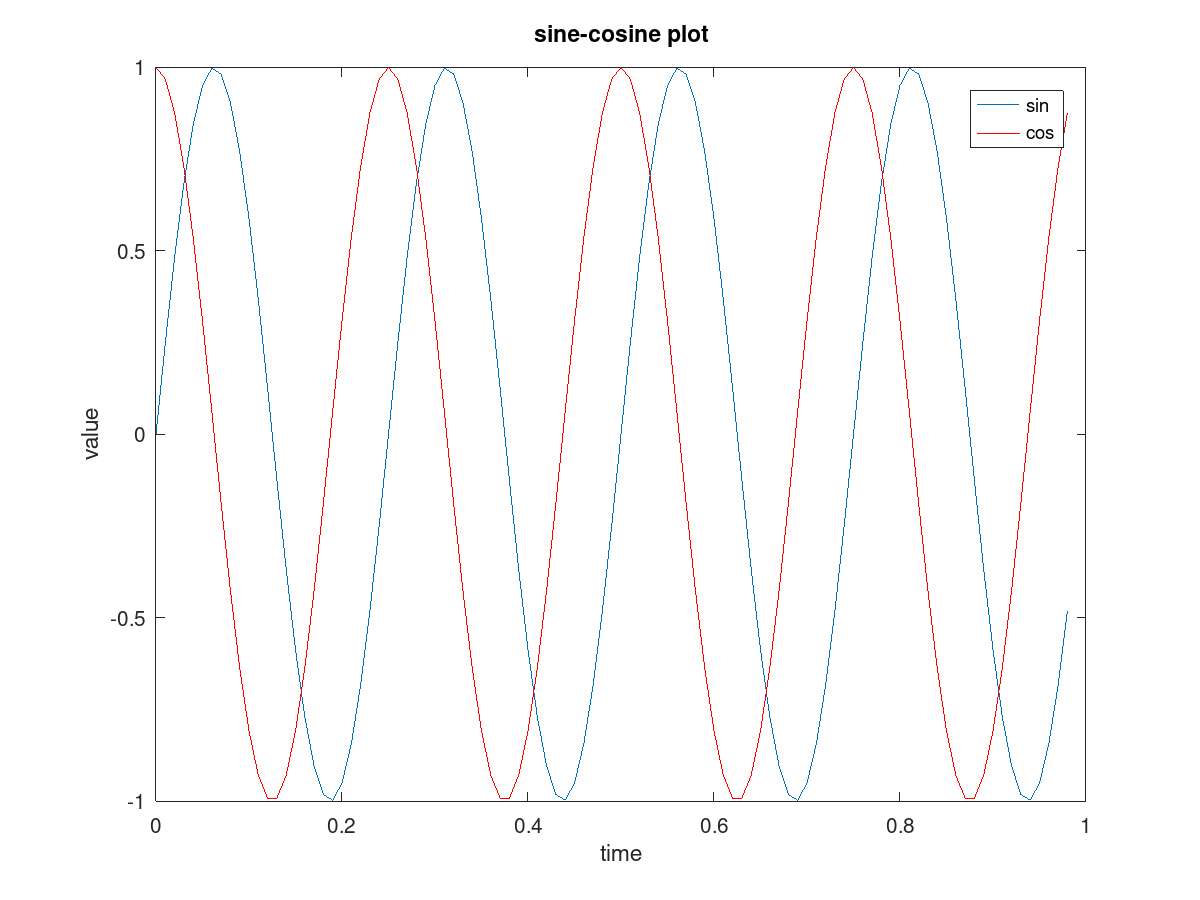
\includegraphics[width=6cm, height=4cm]{myPlot.png}
\end{figure}

\begin{lstlisting}[basicstyle=\small]

octave:13> close
octave:14> figure(1); plot(t, y1);
octave:15> figure(2); plot(t, y2);
octave:16> subplot(1,2,1);   % Divides plot a 1x2 grid
octave:17> plot(t,y1);
octave:18> subplot(1,2,2)
octave:19> plot(t,y2);
octave:20> axis([0.5 1 -1 1])
\end{lstlisting}

\begin{figure}[h]
  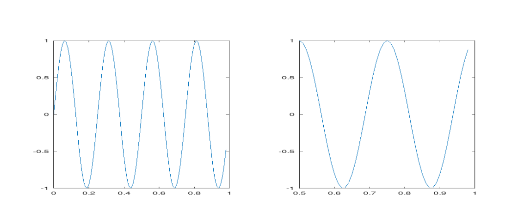
\includegraphics[width=12cm, height=4cm]{plot2.png}
\end{figure}

\vspace{5mm}
\subsubsection{Control Statements: for, while, if, else-if ...}

\begin{lstlisting}[basicstyle=\small]
octave:1> v = zeros(10,1)
v =

   0
   0
   0
   0
   0
   0
   0
   0
   0
   0

octave:2> for i=1:10,
> v(i) = 2^i;
> end;

octave:3> v
v =

      2
      4
      8
     16
     32
     64
    128
    256
    512
   1024

octave:4> i=1;
octave:5> while i <= 5,
> v(i) = 100;
> i = i+1;
> end;
octave:6> v
v =

    100
    100
    100
    100
    100
     64
    128
    256
    512
   1024

octave:7> i = 1;
octave:8> while true,
> v(i) = 999;
> i = i+1;
> if i == 6,
>   break;
> end;
> end;

octave:9> v
v =

    999
    999
    999
    999
    999
     64
    128
    256
    512
   1024

\end{lstlisting}
